%
% $RCSfile: software_engineering_process.tex,v $
%
% Copyright (C) 2002-2008. Christian Heller.
%
% Permission is granted to copy, distribute and/or modify this document
% under the terms of the GNU Free Documentation License, Version 1.1 or
% any later version published by the Free Software Foundation; with no
% Invariant Sections, with no Front-Cover Texts and with no Back-Cover
% Texts. A copy of the license is included in the section entitled
% "GNU Free Documentation License".
%
% http://www.cybop.net
% - Cybernetics Oriented Programming -
%
% http://www.resmedicinae.org
% - Information in Medicine -
%
% Version: $Revision: 1.1 $ $Date: 2008-08-19 20:41:08 $ $Author: christian $
% Authors: Christian Heller <christian.heller@tuxtax.de>
%

\chapter{Software Engineering Process}
\label{software_engineering_process_heading}
\index{Software Engineering Process}
\index{SEP}
\index{Lifecycle of Software}
\index{Software Lifecycle}
\index{Waterfall Process}
\index{Iterative Process}
\index{Agile Software Development}
\index{Extreme Programming}
\index{Abstractions}
\index{Requirements Analysis Document}
\index{Architecture Design Diagrams}
\index{Implementation Source Code}

\begin{flushright}
    \textsl{The Way is the Aim.}\\
    \textsc{Confucius}
\end{flushright}

Software does not only contain and process information, it is information itself.
Its creation, existence, growing old and death are called \emph{Lifecycle}.
Software stands at the end of a sequence of abstractions which is often called a
\emph{Software Engineering Process} (SEP). Besides the single steps of work and
methodology to follow, a SEP often specifies the tools to be used and the roles
of people involved \cite{balzert}. Software development history has shown plenty
of different forms of such processes, but most can be categorised into one of
the following:

\begin{itemize}
    \item[-] Waterfall Process
    \item[-] Iterative Process
    \item[-] Agile Software Development
    \item[-] Extreme Programming
\end{itemize}

This work is not exactly about software engineering processes, nor does it want
to introduce yet another one. Its main purpose is to deal with the results of a
SEP's phases: \emph{Abstractions}. Three forms of abstraction are common to most
processes:

\begin{itemize}
    \item[-] Requirements Analysis Document
    \item[-] Architecture Design Diagrams
    \item[-] Implementation Source Code
\end{itemize}

In order to have a common base of understanding and to be able to estimate the
effects of abstraction changes on the actual software development phases, it is
necessary to briefly describe some processes, which is done in the following
sections.

%
% $RCSfile: waterfall_process.tex,v $
%
% Copyright (C) 2002-2008. Christian Heller.
%
% Permission is granted to copy, distribute and/or modify this document
% under the terms of the GNU Free Documentation License, Version 1.1 or
% any later version published by the Free Software Foundation; with no
% Invariant Sections, with no Front-Cover Texts and with no Back-Cover
% Texts. A copy of the license is included in the section entitled
% "GNU Free Documentation License".
%
% http://www.cybop.net
% - Cybernetics Oriented Programming -
%
% http://www.resmedicinae.org
% - Information in Medicine -
%
% Version: $Revision: 1.1 $ $Date: 2008-08-19 20:41:09 $ $Author: christian $
% Authors: Christian Heller <christian.heller@tuxtax.de>
%

\section{Waterfall Process}
\label{waterfall_process_heading}
\index{Waterfall Process}
\index{Requirements}
\index{Analysis}
\index{Design}
\index{Implementation}
\index{Test}
\index{Integration}
\index{Back Flow of Waterfall Process}
\index{V-Model}
\index{V-Modell 97}
\index{Big Bang Delivery}

The \emph{Waterfall Process} (figure \ref{waterfall_figure}) is the classical
way to develop a product. It assumes that the requirements are clear and do not
change during a project. Waterfall software development is pretty straightforward
and usually consists of the sequenced phases \emph{Requirements}, \emph{Analysis},
\emph{Design}, \emph{Implementation} (Realisation, Coding), \emph{Test} and
\emph{Integration} (Release).

\begin{figure}[ht]
    \begin{center}
        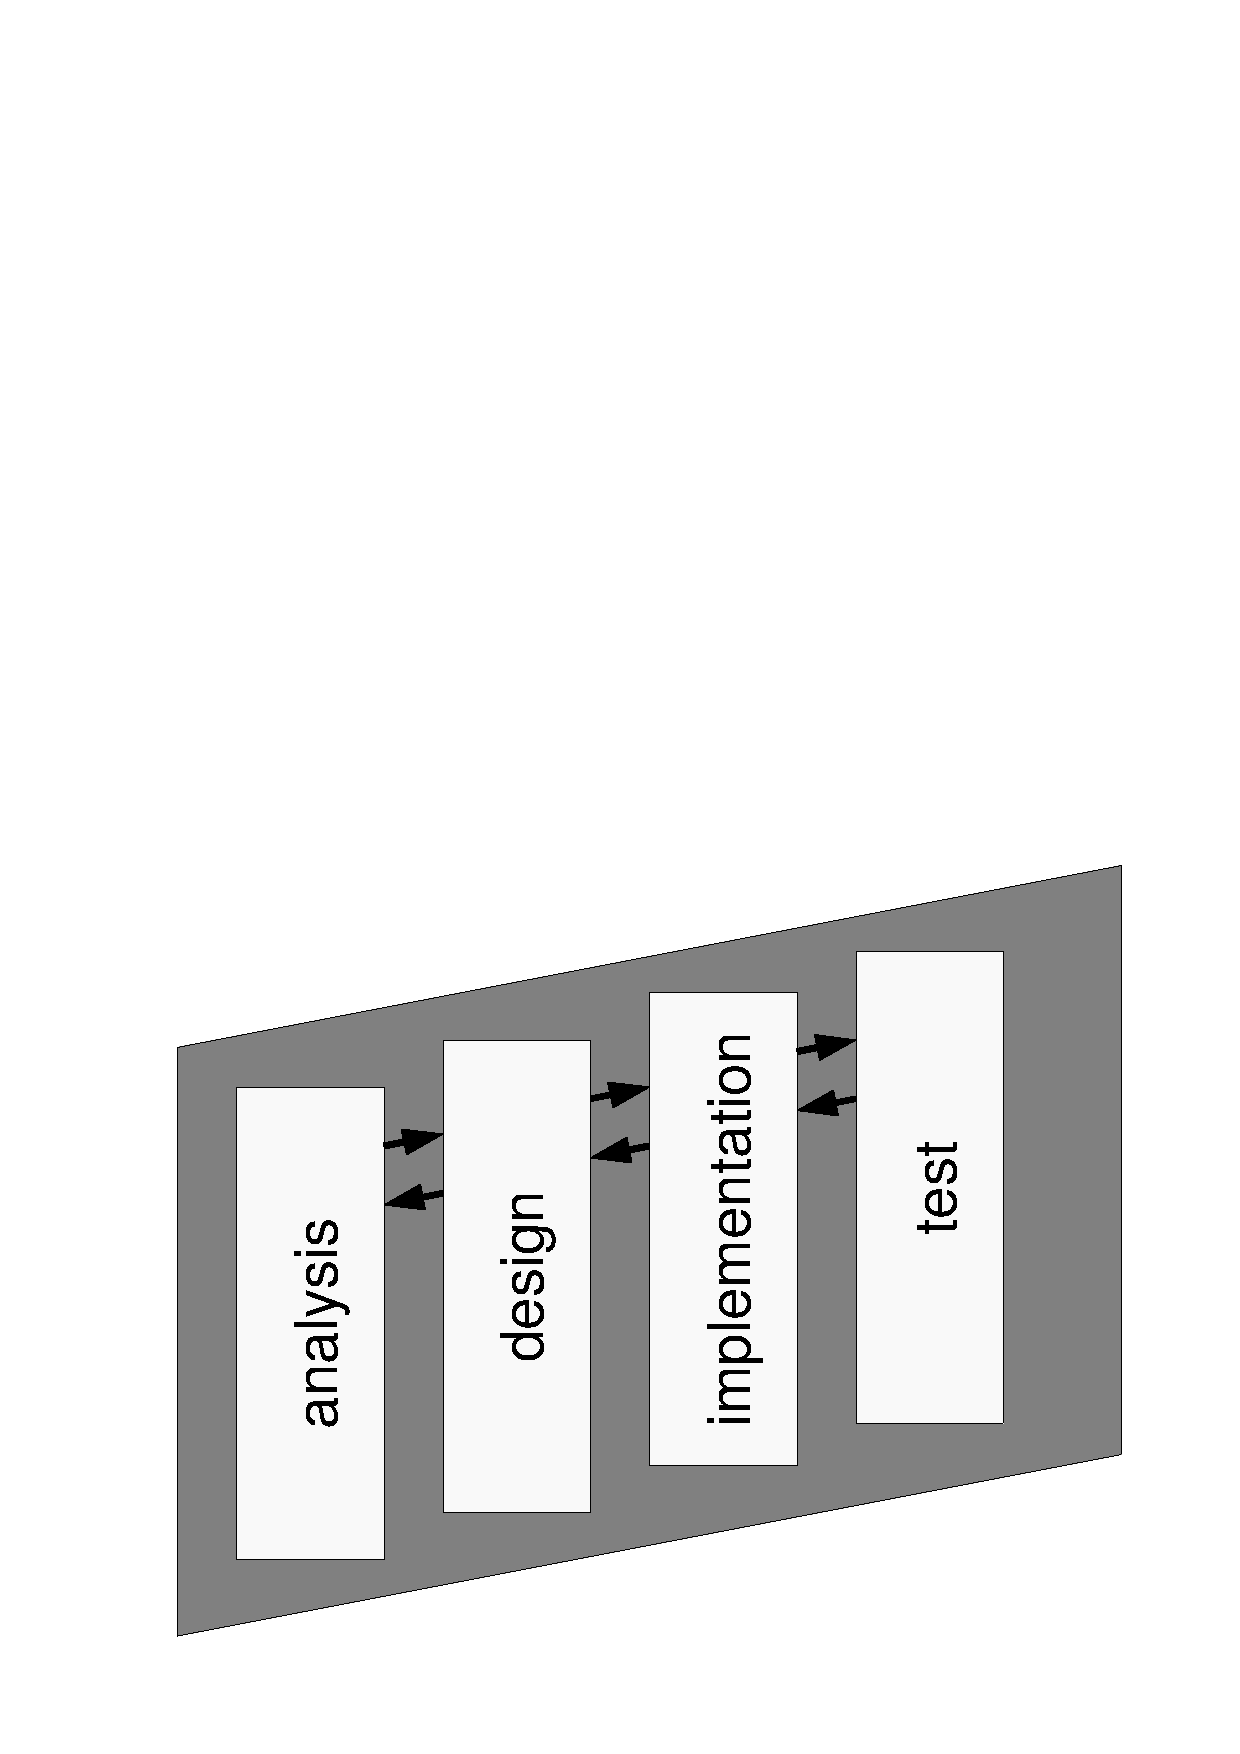
\includegraphics[scale=0.3,angle=-90]{graphic/waterfall.pdf}
        \caption{Waterfall Process with Back Flow}
        \label{waterfall_figure}
    \end{center}
\end{figure}

\begin{figure}[ht]
    \begin{center}
        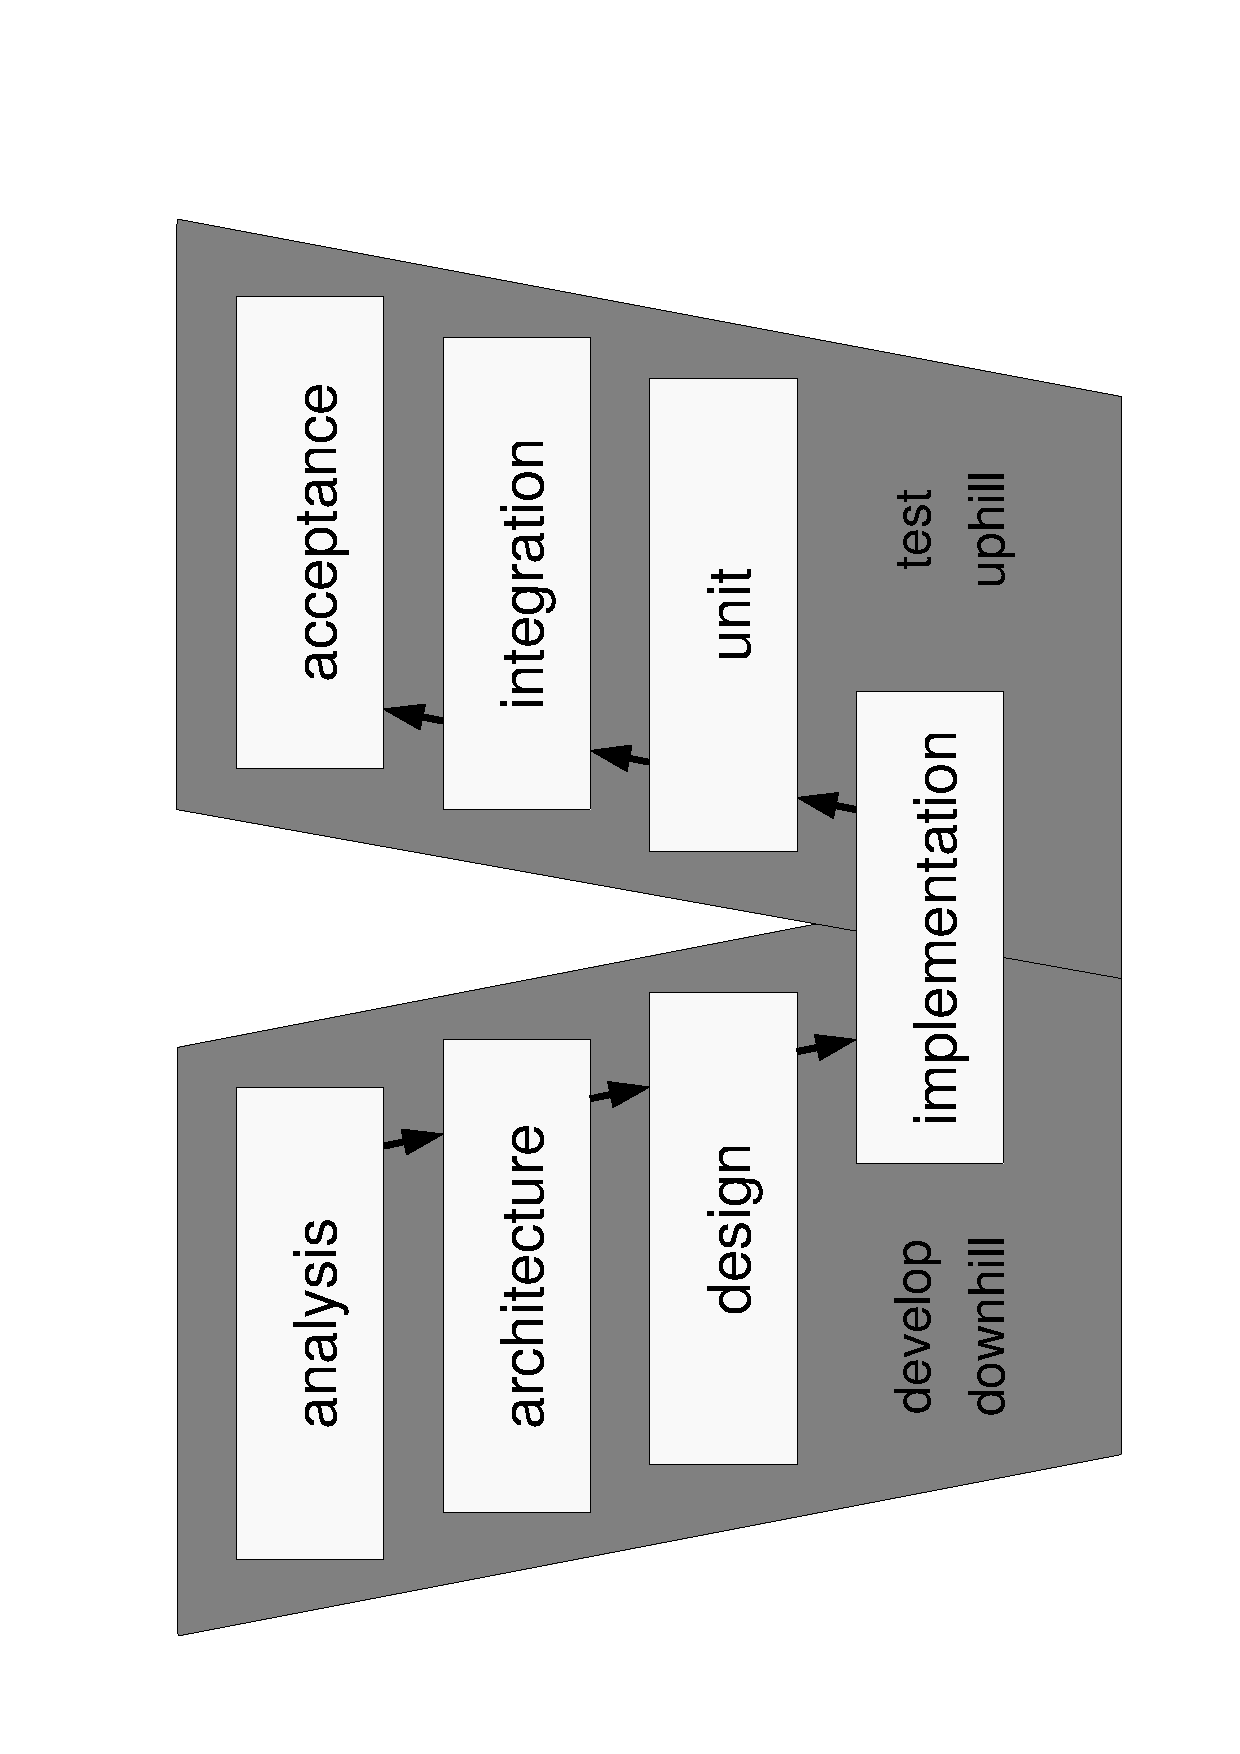
\includegraphics[scale=0.3,angle=-90]{graphic/vmodel.pdf}
        \caption{V-Model}
        \label{vmodel_figure}
    \end{center}
\end{figure}

Numerous variations of waterfall processes exist. The simplest ones deliver
their product at once, at the end of the project, what is often called
\emph{Big Bang Delivery} \cite{malotaux}. Others integrate some kind of
\emph{Back Flow} \cite{sweedyk} that allows to consider test results in further
development. One example that has combined software development- and testing
activities is the \emph{V-Modell 97} \cite{vmodel} (figure \ref{vmodel_figure}).
Its name stands for its shape: the left-hand (downhill) side of the \emph{V}
represents the development; the right-hand (uphill) side represents the
corresponding test activities.

%
% $RCSfile: iterative_process.tex,v $
%
% Copyright (C) 2002-2008. Christian Heller.
%
% Permission is granted to copy, distribute and/or modify this document
% under the terms of the GNU Free Documentation License, Version 1.1 or
% any later version published by the Free Software Foundation; with no
% Invariant Sections, with no Front-Cover Texts and with no Back-Cover
% Texts. A copy of the license is included in the section entitled
% "GNU Free Documentation License".
%
% http://www.cybop.net
% - Cybernetics Oriented Programming -
%
% http://www.resmedicinae.org
% - Information in Medicine -
%
% Version: $Revision: 1.1 $ $Date: 2008-08-19 20:41:07 $ $Author: christian $
% Authors: Christian Heller <christian.heller@tuxtax.de>
%

\section{Iterative Process}
\label{iterative_process_heading}
\index{Iterative Process}
\index{Reentrant Structure}
\index{Feedback Loop}
\index{Incremental Process}
\index{Evolutionary Process}
\index{Staged Process}
\index{Spiral Process}
\index{Whirlpool Process}
\index{Rational Unified Process}
\index{RUP}
\index{Unified Modeling Language}
\index{UML}

An \emph{Iterative Process} (figure \ref{iterative_figure}) contains phases
as known from the waterfall process, supplemented by the new idea of a
\emph{Reentrant Structure} (\emph{Feedback Loop}). All phases are gone through
repeatedly, as long as the product is not satisfying. Whenever new requirements
show up, also after completion, new features can be added to the system by
reiterating a new project cycle.

\begin{figure}[ht]
    \begin{center}
        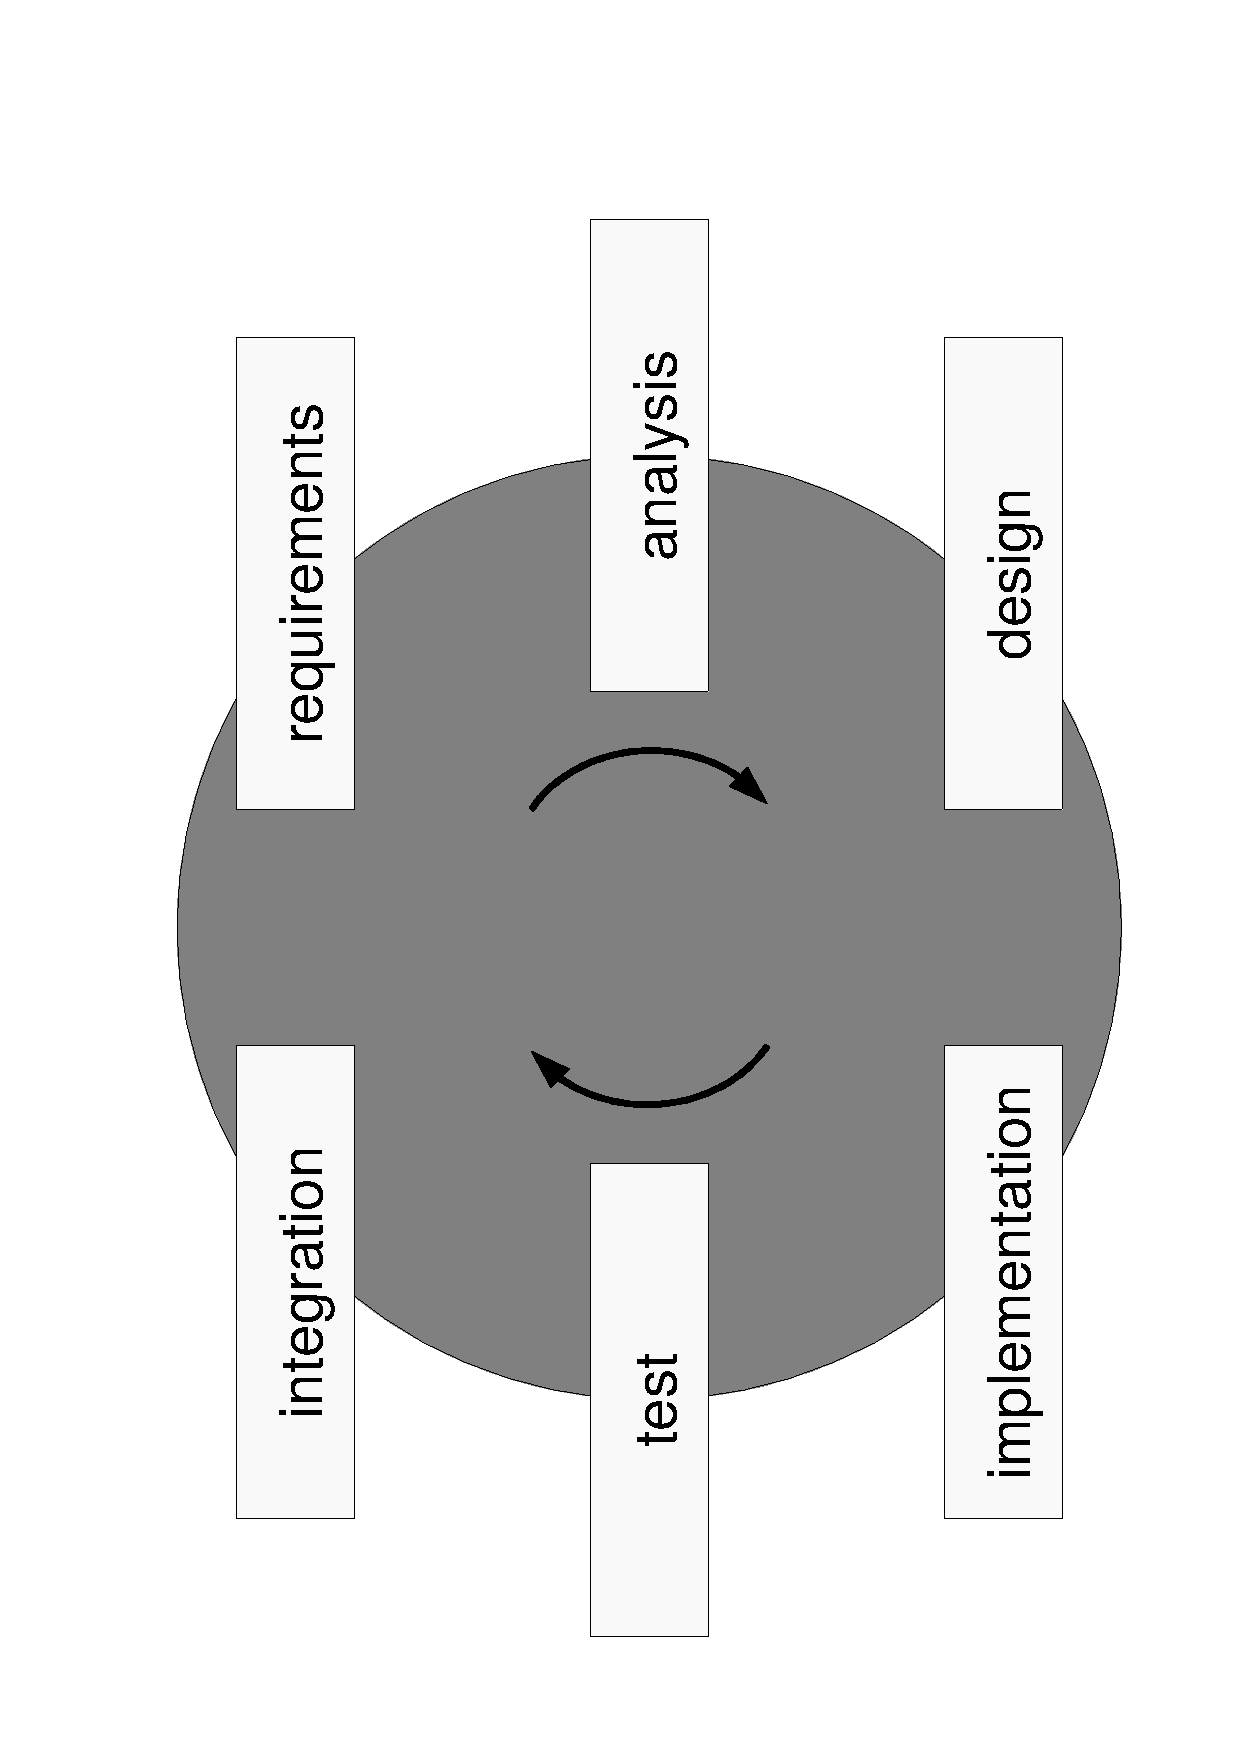
\includegraphics[scale=0.3,angle=-90]{graphic/iterative.pdf}
        \caption{Iterative Process}
        \label{iterative_figure}
    \end{center}
\end{figure}

Also here, many variations exist. They are called \emph{incremental},
\emph{evolutionary}, \emph{staged}, \emph{spiral} or \emph{whirlpool}, or
similarly. In the end, they all have their roots in some kind of
\emph{Iteration} which should \textit{frequently produce working versions of
the final system that have a subset of the required features}, as Fowler
\cite{fowlernewmethodology} writes.

A famous representative is the \emph{Rational Unified Process} (RUP) \cite{rup}.
Developed by Philippe Kruchten, Ivar Jacobson and others, RUP is the process
complement to the \emph{Unified Modeling Language} (UML). Its strength of being
a process framework that can accommodate a wide variety of processes is its
weakness, at the same time. Fowler \cite{fowlernewmethodology} criticises this
as follows:

\begin{quote}
    As a result of this process framework mentality, RUP can be used in a very
    traditional waterfall style or in an agile manner (explained in section
    \ref{agile_methodologies_heading}). So as a result you can use RUP as an
    agile process, or as a heavyweight process -- it all depends on how you
    tailor it in your environment.
\end{quote}

%
% $RCSfile: agile_methodologies.tex,v $
%
% Copyright (C) 2002-2008. Christian Heller.
%
% Permission is granted to copy, distribute and/or modify this document
% under the terms of the GNU Free Documentation License, Version 1.1 or
% any later version published by the Free Software Foundation; with no
% Invariant Sections, with no Front-Cover Texts and with no Back-Cover
% Texts. A copy of the license is included in the section entitled
% "GNU Free Documentation License".
%
% http://www.cybop.net
% - Cybernetics Oriented Programming -
%
% http://www.resmedicinae.org
% - Information in Medicine -
%
% Version: $Revision: 1.1 $ $Date: 2008-08-19 20:41:05 $ $Author: christian $
% Authors: Christian Heller <christian.heller@tuxtax.de>
%

\section{Agile Methodologies}
\label{agile_methodologies_heading}
\index{Agile Methodologies}
\index{Agile Manifesto}
\index{Extreme Programming}
\index{XP}
\index{Open Source Software}
\index{OSS}
\index{Crystal Family}
\index{Adaptive Software Development}
\index{ASD}
\index{Scrum}
\index{Feature Driven Development}
\index{FDD}
\index{Dynamic System Development Method}
\index{DSDM}
\index{Context Driven Testing}
\index{Agile Alliance}

The principles of \emph{Agile Methodologies} (figure \ref{agile_figure}) are
applied by a group of so-called \emph{lightweight}, \emph{adaptive} software
development processes with few bureaucracy, less predictability, less process-
and document-orientation, but more emphasis on people and their skills, and on
source code -- which is considered the key part of documentation.

\begin{figure}[ht]
    \begin{center}
        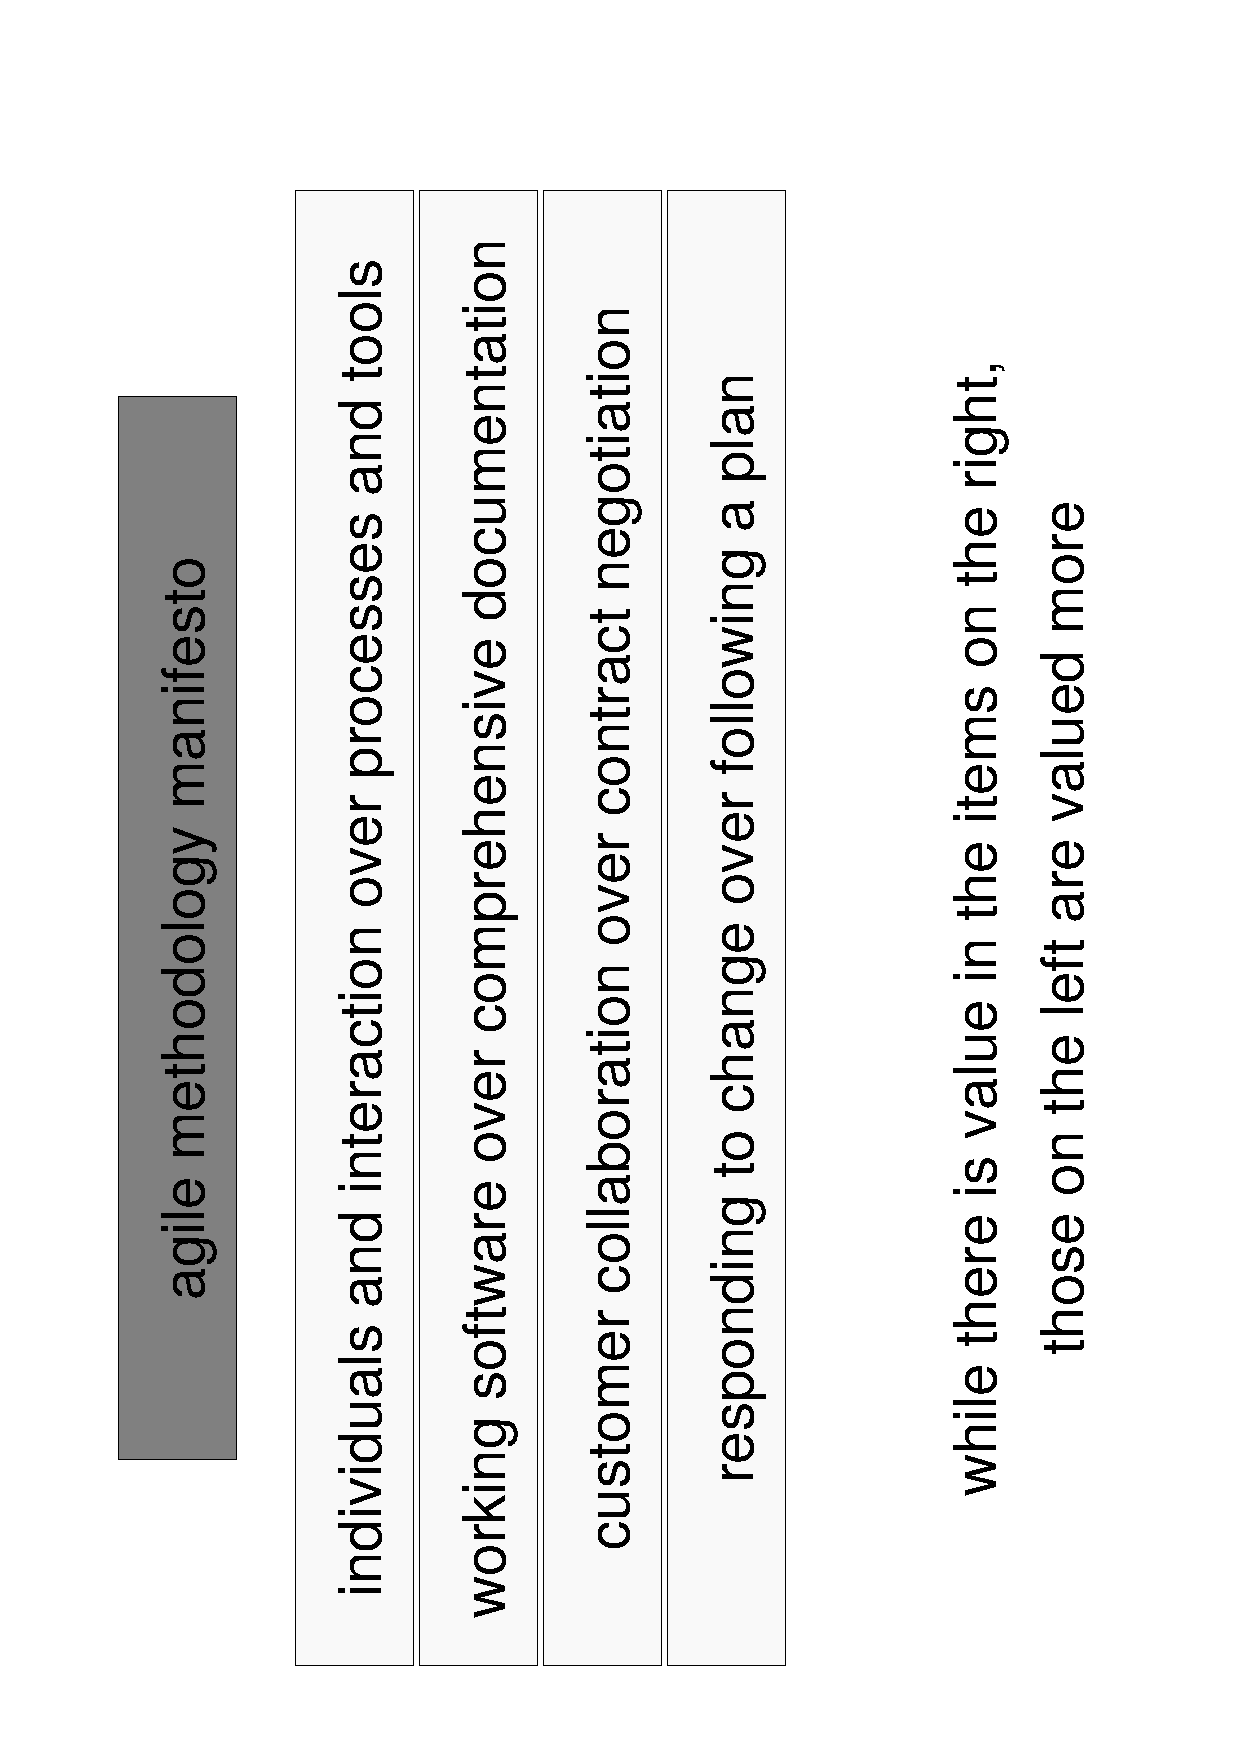
\includegraphics[scale=0.3,angle=-90]{graphic/agile.pdf}
        \caption{Agile Manifesto}
        \label{agile_figure}
    \end{center}
\end{figure}

Besides \emph{Extreme Programming} (XP) and \emph{Open Source Software} (OSS)
development, both described in section \ref{extreme_programming_heading}, there
are several other methodologies that fit under the \emph{Agile} banner. Fowler
explains some of them in \cite{fowlernewmethodology}, which contains Alistair
Cockburn's \emph{Crystal Family}, Jim Highsmith's
\emph{Adaptive Software Development} (ASD), \emph{Scrum},
\emph{Feature Driven Development} (FDD) by Jeff De Luca and Peter Coad, the
\emph{Dynamic System Development Method} (DSDM) specified by a consortium of
British companies and some remarks on \emph{Context Driven Testing}.

For the purpose of this paper, further investigation on details of the
mentioned methodologies is not needed. The general principles of agile software
development (manifesto) are the important part to recognise, because they
suggest a different, more \emph{agile} approach to software engineering.
Although many techniques of agile methodologies had been known and used for
long, at least in OSS development, they had not been investigated, documented
and promoted for business use in this form before. This is the great
achievement of the \emph{Agile Alliance} \cite{agilealliance}.

%
% $RCSfile: extreme_programming.tex,v $
%
% Copyright (C) 2002-2008. Christian Heller.
%
% Permission is granted to copy, distribute and/or modify this document
% under the terms of the GNU Free Documentation License, Version 1.1 or
% any later version published by the Free Software Foundation; with no
% Invariant Sections, with no Front-Cover Texts and with no Back-Cover
% Texts. A copy of the license is included in the section entitled
% "GNU Free Documentation License".
%
% http://www.cybop.net
% - Cybernetics Oriented Programming -
%
% http://www.resmedicinae.org
% - Information in Medicine -
%
% Version: $Revision: 1.1 $ $Date: 2008-08-19 20:41:06 $ $Author: christian $
% Authors: Christian Heller <christian.heller@tuxtax.de>
%

\section{Extreme Programming}
\label{extreme_programming_heading}
\index{Extreme Programming}
\index{XP}
\index{Iterative Structure}
\index{Iteration in XP}
\index{Development in XP}
\index{Collective Code Ownership in XP}
\index{User Stories}
\index{Release Planning}
\index{Learn and Communicate}
\index{Stand Up Meeting}
\index{Free and Open Source Software}
\index{FOSS}
\index{The Cathedral and the Bazar}

\emph{Extreme Programming} (XP) uses the idea of an iterative structure as
explained in section \ref{iterative_process_heading}, with the difference that
it contains not only one but many cycles to assure sufficient feedback. The whole
process can be cascaded and split into more fine-grained processes, for example
\emph{Iteration}, \emph{Development} and \emph{Collective Code Ownership}.
Figure \ref{xp_figure} shows a strongly simplified view of the XP methodology,
with emphasis on its nested structure and multiple iterations. Better and more
detailed overviews are given in \cite{xp}.

\begin{figure}[ht]
    \begin{center}
        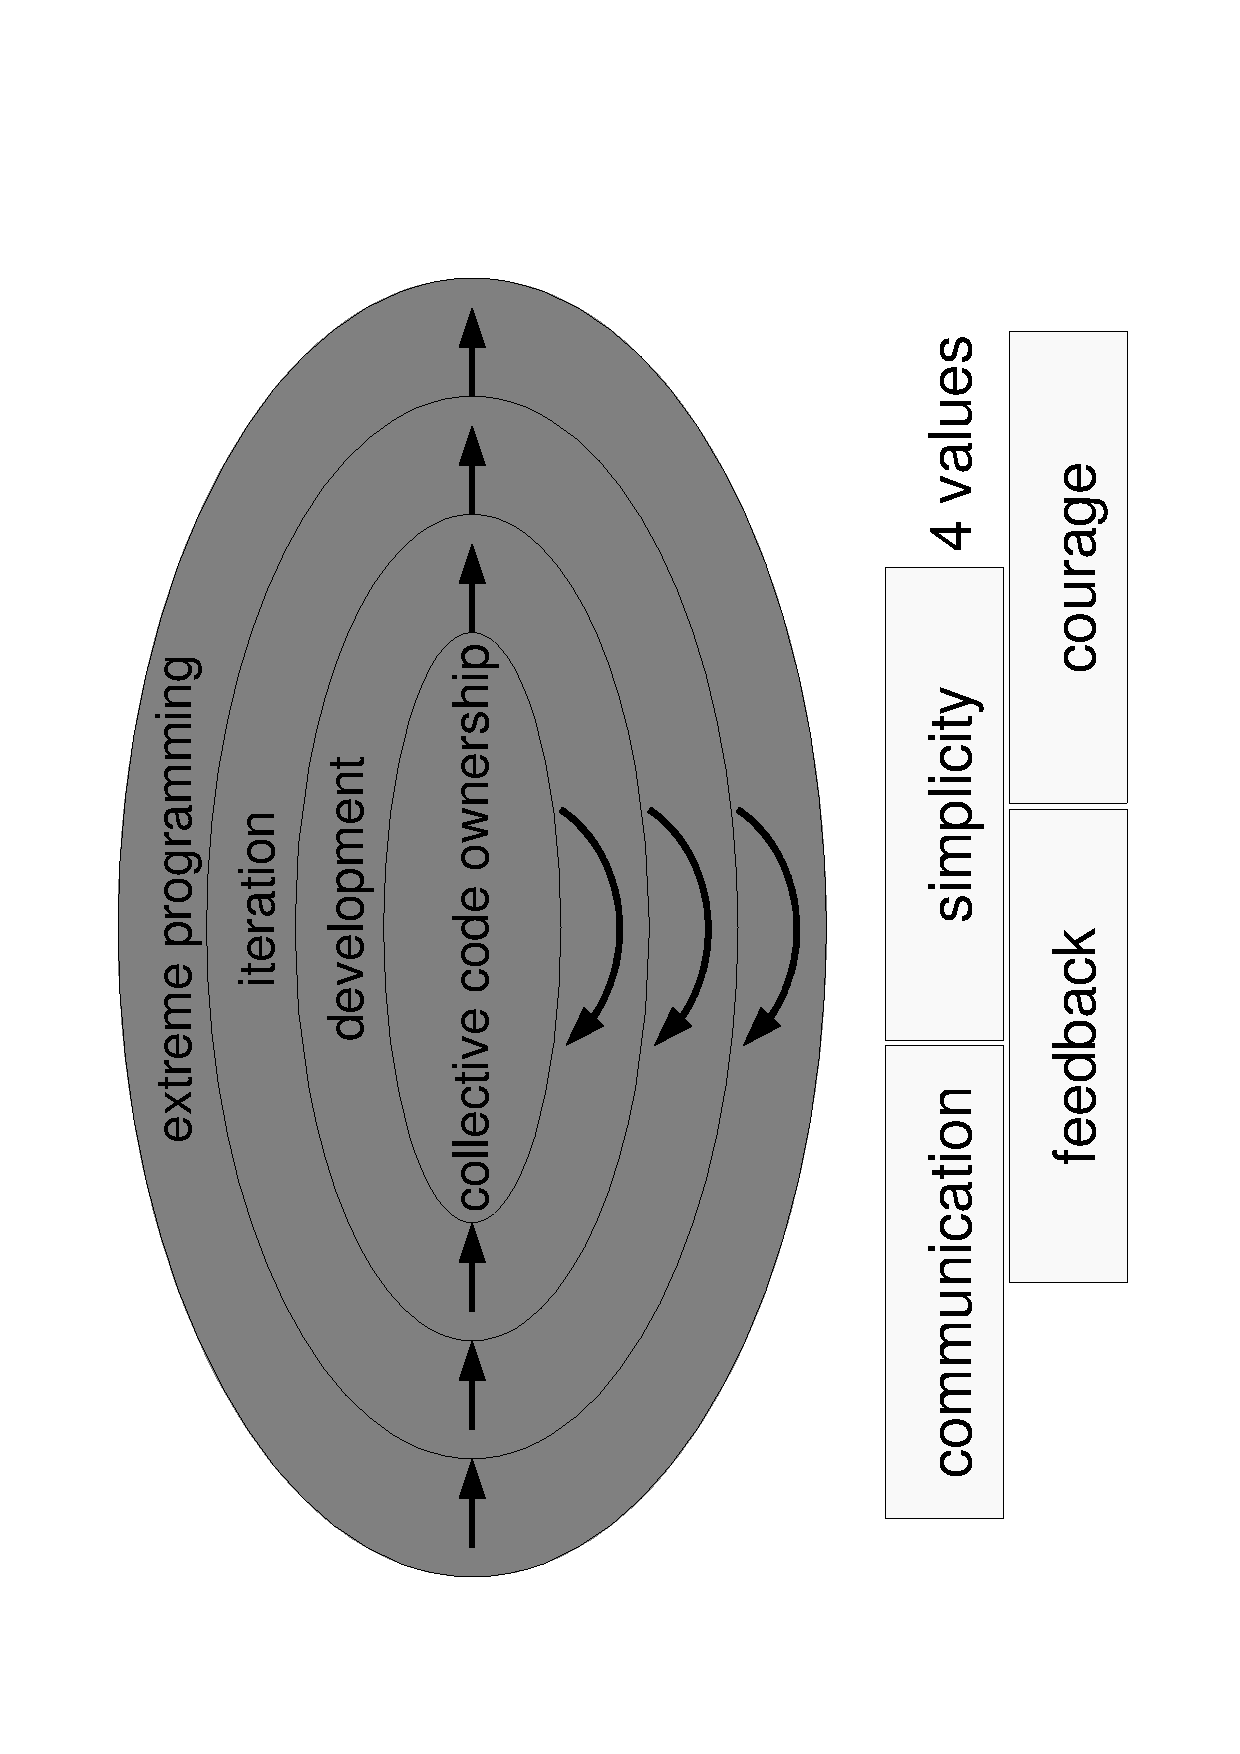
\includegraphics[scale=0.3,angle=-90]{graphic/xp.pdf}
        \caption{Extreme Programming (strongly simplified)}
        \label{xp_figure}
    \end{center}
\end{figure}

In some way or the other, the classical process phases as first mentioned in
section \ref{waterfall_process_heading} also appear in XP, although they may
have different names or a modified meaning. The requirements document, for
example, is replaced by so-called \emph{User Stories}, which are similar to
usage scenarios (except that they are not limited to describing a user
interface), but not to be mixed up with use cases \cite{xp}. Also, a number of
new phases like \emph{Release Planning} appear and more fine-granular
activities like \emph{Learn and Communicate} or \emph{Stand Up Meeting} are
added. The basis and starting point of each XP project are four common values:

\begin{itemize}
    \item[-] Communication
    \item[-] Feedback
    \item[-] Simplicity
    \item[-] Courage
\end{itemize}

The last decade has shown several pushes and increasingly greater support for
\emph{Free and Open Source Software} (FOSS) \cite{opensource}. What makes this
software so successful, besides the fact that its source code is open and
freely available, is its astonishingly fast development model. Well, there
surely are as many different development methodologies as there are FOSS
projects out there, but many of them would probably, at least partly,
match into XP. Additionally, however, there are a few significant differences
that characterise \emph{Open Source Development}. Among them are
\cite{fowlernewmethodology}:

\begin{itemize}
    \item[-] Collaboration between physically distributed teams
    \item[-] Maintainer responsible for overall coordination and design
    \item[-] Highly parallelisable debugging
\end{itemize}

In his book \emph{The Cathedral and the Bazar} \cite{raymond}, Eric S. Raymond
provides further insights. Popular slogans taken from it are: \textit{Release
early and often!}, \textit{Delegate everything you can!} or: \textit{Be open to
the point of promiscuity!} He recommends to foster a community of developers,
lead by \emph{Doing} and \emph{Good Humour}. Yet Tim Churches reminds people not
to take Raymond's recommendations as dogma \cite{openhealth}:

\begin{quote}
    Although Eric S. Raymond's \ldots\ essay brought one particular FOSS
    development paradigm to a lot of people's attention, it may have also done
    the FOSS movement a disservice by making people think that the 'bazaar'
    approach is the only way in which FOSS can be developed.
\end{quote}

Instead, each project should pick a methodology that best suits its needs, may
it be cathedral- or bazaar-like.

%
% $RCSfile: method_maturity.tex,v $
%
% Copyright (C) 2002-2008. Christian Heller.
%
% Permission is granted to copy, distribute and/or modify this document
% under the terms of the GNU Free Documentation License, Version 1.1 or
% any later version published by the Free Software Foundation; with no
% Invariant Sections, with no Front-Cover Texts and with no Back-Cover
% Texts. A copy of the license is included in the section entitled
% "GNU Free Documentation License".
%
% http://www.cybop.net
% - Cybernetics Oriented Programming -
%
% http://www.resmedicinae.org
% - Information in Medicine -
%
% Version: $Revision: 1.1 $ $Date: 2008-08-19 20:41:07 $ $Author: christian $
% Authors: Christian Heller <christian.heller@tuxtax.de>
%

\section{Method Maturity}
\label{method_maturity_heading}
\index{Method Maturity}
\index{Capability Maturity Model for Software}
\index{SW-CMM}
\index{Capability Maturity Model Integration}
\index{CMMI}
\index{V-Model}
\index{Extreme Programming}
\index{XP}

Numerous research efforts try to find the ideal software development paradigm and
many academic papers were written on the topic. In order to be able to compare
the resulting methodologies, a couple of which were described in the previous
sections, some kind of measure is needed.

The \emph{Capability Maturity Model for Software} (SW-CMM) \cite{paulk} is such
a measure. The newer CMM version is called
\emph{Capability Maturity Model Integration} (CMMI). Intended to help
organisations improve the maturity of their software processes, it describes
underlying principles and practices in terms of an evolutionary path
\cite{cmm}. The CMM is organised into five levels describing a software
process' maturity:

\begin{enumerate}
    \item \emph{Initial:} ad hoc, occasionally even chaotic, scarcely defined
    \item \emph{Repeatable:} established discipline for repetition of earlier successes
    \item \emph{Defined:} documented, standardised activities for organisation
    \item \emph{Managed:} detailed quality measures, quantitative understanding
    \item \emph{Optimising:} continuous improvement through feedback
\end{enumerate}

Two examples using the CMM for process evaluation are described in
\cite{schuppan} which considers the \emph{V-Model} and in \cite{paulkxp} which
investigates \emph{XP}.

%
% $RCSfile$
%
% Copyright (c) 2005-2006. Christian Heller. All rights reserved.
%
% Permission is granted to copy, distribute and/or modify this document
% under the terms of the GNU Free Documentation License, Version 1.1 or
% any later version published by the Free Software Foundation; with no
% Invariant Sections, with no Front-Cover Texts and with no Back-Cover
% Texts. A copy of the license is included in the section entitled
% "GNU Free Documentation License".
%
% http://www.cybop.net
% - Cybernetics Oriented Programming -
%
% http://www.resmedicinae.org
% - Information in Medicine -
%
% Version: $Revision$ $Date$ $Author$
% Authors: Christian Heller <christian.heller@tuxtax.de>
%

\subsection{Abstraction Gaps}
\label{abstraction_gaps_heading}

Software has to be developed in a creative process called
\emph{Software Engineering Process} (SEP) or \emph{Methodology} (figure
\ref{gaps_figure}).

\begin{figure}[htb]
    \begin{center}
        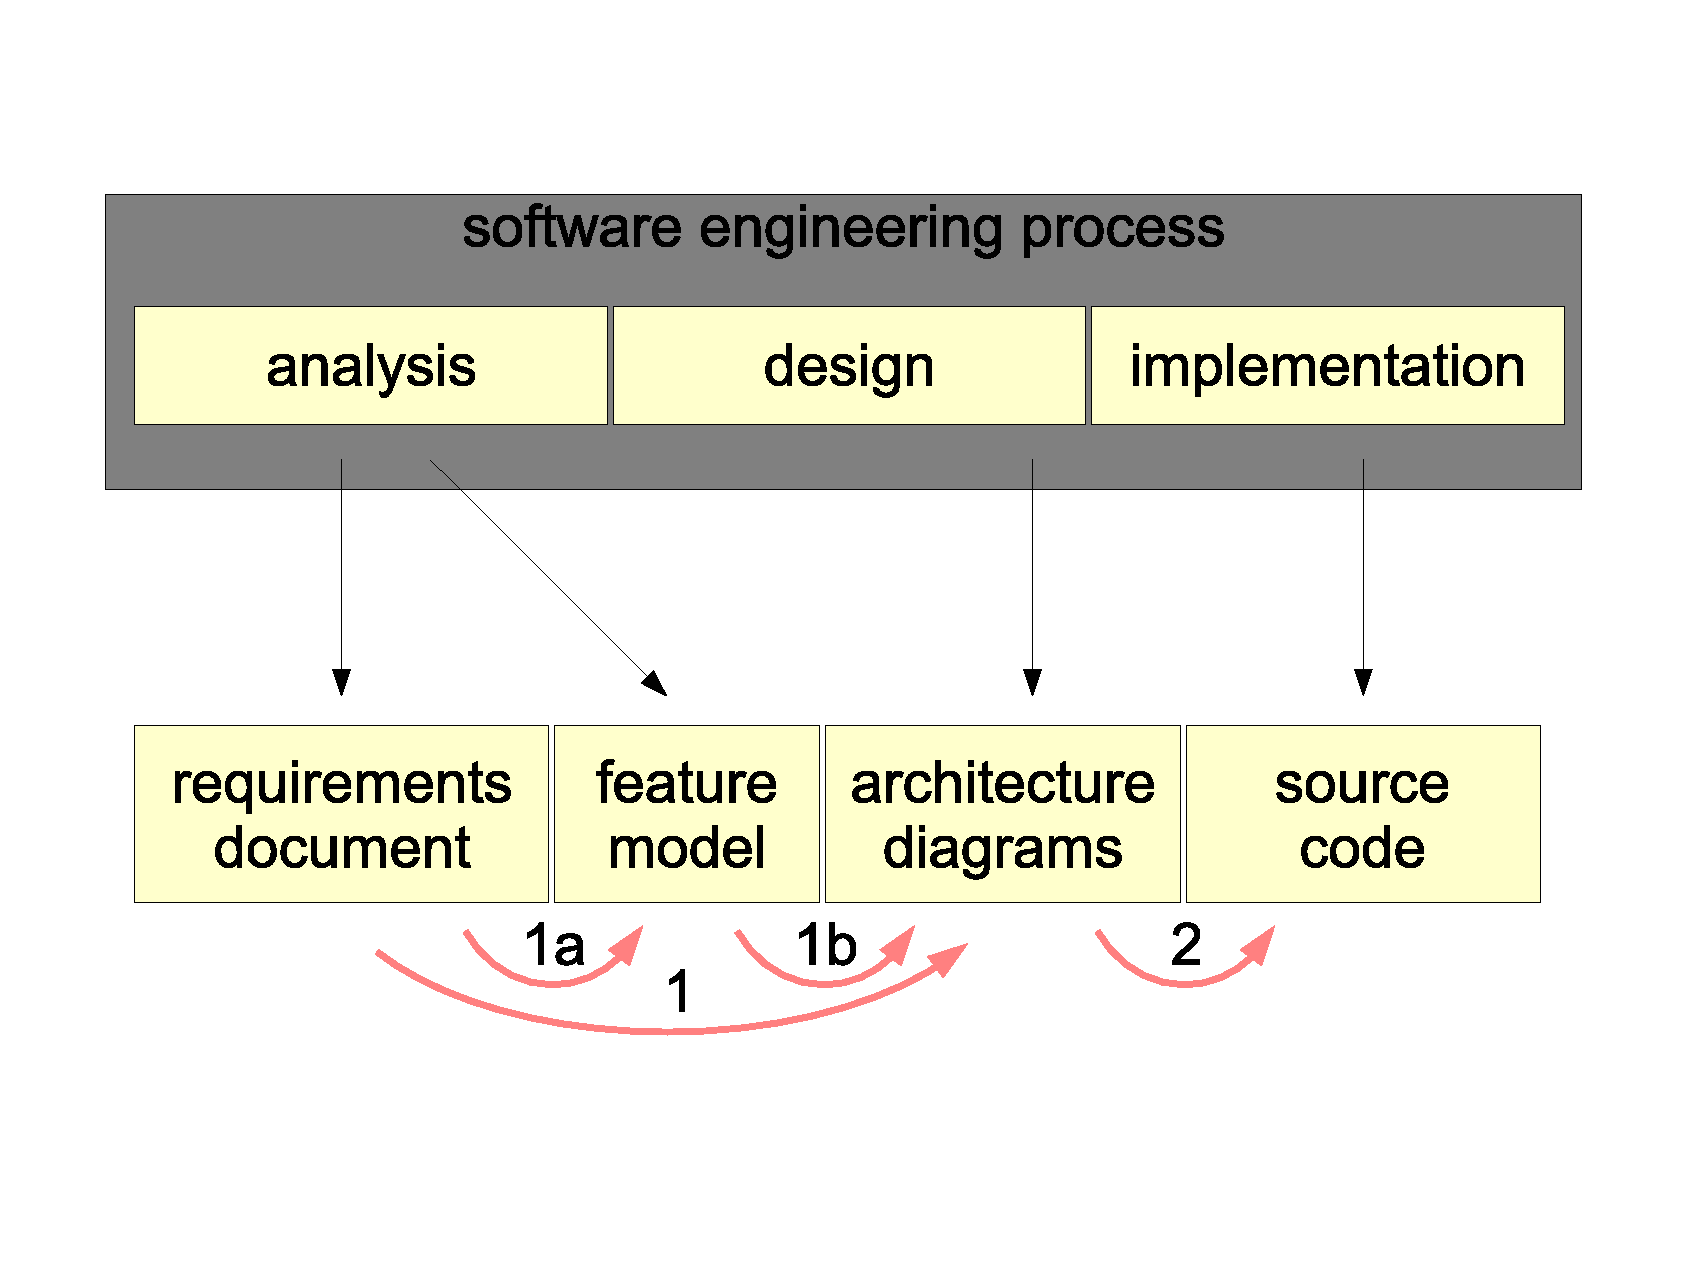
\includegraphics[scale=0.2]{vector/gaps.eps}
        \caption{Abstraction Gaps}
        \label{gaps_figure}
    \end{center}
\end{figure}

Different forms of SEP exist: \emph{Waterfall}, \emph{Iterative},
\emph{Extreme Programming} (XP) and \emph{Agile Programming}. But every
project, consciously or not, follows a SEP that sooner-or-later, in one form or
the other, goes through three common phases: \emph{Analysis}, \emph{Design} and
\emph{Implementation}. Each phase creates its own model of what is to be
abstracted in software and it is the differences in exactly these models that
often cause complications.

A previous article \cite{heller2004} mentioned the \emph{Requirements Document},
\emph{Feature Model}, \emph{Architecture Diagrams} and \emph{Source Code} as
forms of knowledge abstraction. It also described the following abstraction
gaps (see figure \ref{gaps_figure}) that have to be crossed:

\begin{enumerate}
    \item[1a] Requirements Document/Feature M.
    \item[1b] Feature Model/Architecture Diagr.
    \item[2] Architecture Diagrams/Source Code
\end{enumerate}

By improving the \emph{Traceability} between requirements and the architecture,
feature models (known from system family/ product line engineering) contribute
to minimising gap 1. Together with architecture diagrams, they ease
communication between stakeholders in the SEP, because of their human-readable
form and implementation-independence. But sooner-or-later, also these have to
be transferred into source code, by crossing gap 2.

Bridging or closing these abstraction gaps (sometimes called \emph{Semantic- or
Conceptual Gaps}) is also known as: \textit{achieving higher intentionality}
and remains an unsolved task for software engineering. One aim of the work
described in this article was to contribute to a possible solution, with focus
on \emph{reducing} gap 2, existing between a designed architecture and the
implemented code.

%
% $RCSfile: software_architecture.tex,v $
%
% Copyright (C) 2002-2008. Christian Heller.
%
% Permission is granted to copy, distribute and/or modify this document
% under the terms of the GNU Free Documentation License, Version 1.1 or
% any later version published by the Free Software Foundation; with no
% Invariant Sections, with no Front-Cover Texts and with no Back-Cover
% Texts. A copy of the license is included in the section entitled
% "GNU Free Documentation License".
%
% http://www.cybop.net
% - Cybernetics Oriented Programming -
%
% http://www.resmedicinae.org
% - Information in Medicine -
%
% Version: $Revision: 1.1 $ $Date: 2008-08-19 20:41:08 $ $Author: christian $
% Authors: Christian Heller <christian.heller@tuxtax.de>
%

\section{Software Architecture}
\label{software_architecture_heading}
\index{Software Architecture}
\index{Architecture Views}
\index{Four Views Model}
\index{Conceptual View}
\index{Module View}
\index{Code View}
\index{Execution View}
\index{4+1 View Model of Architecture}
\index{Rational Unified Process}
\index{RUP}
\index{Logical View}
\index{Design View}
\index{Development View}
\index{Implementation View}
\index{Physical View}
\index{Deployment View}
\index{Process View}
\index{Scenarios}
\index{Use Case +1 View}
\index{Architecture Description Languages}
\index{ADL}

As was shown in the previous sections, a software engineering process covers a
whole spectrum of activities and abstractions. Several models were created to gain
an \emph{overall} view on the resulting system architectures, across the single
software development phases. The so-called \emph{Architecture Views} that these
models provide represent \textit{a whole system from the perspective of a related
set of concerns}, as \cite{ieee1471-2000} states. Two examples are shown following.

\begin{figure}[ht]
    \begin{center}
        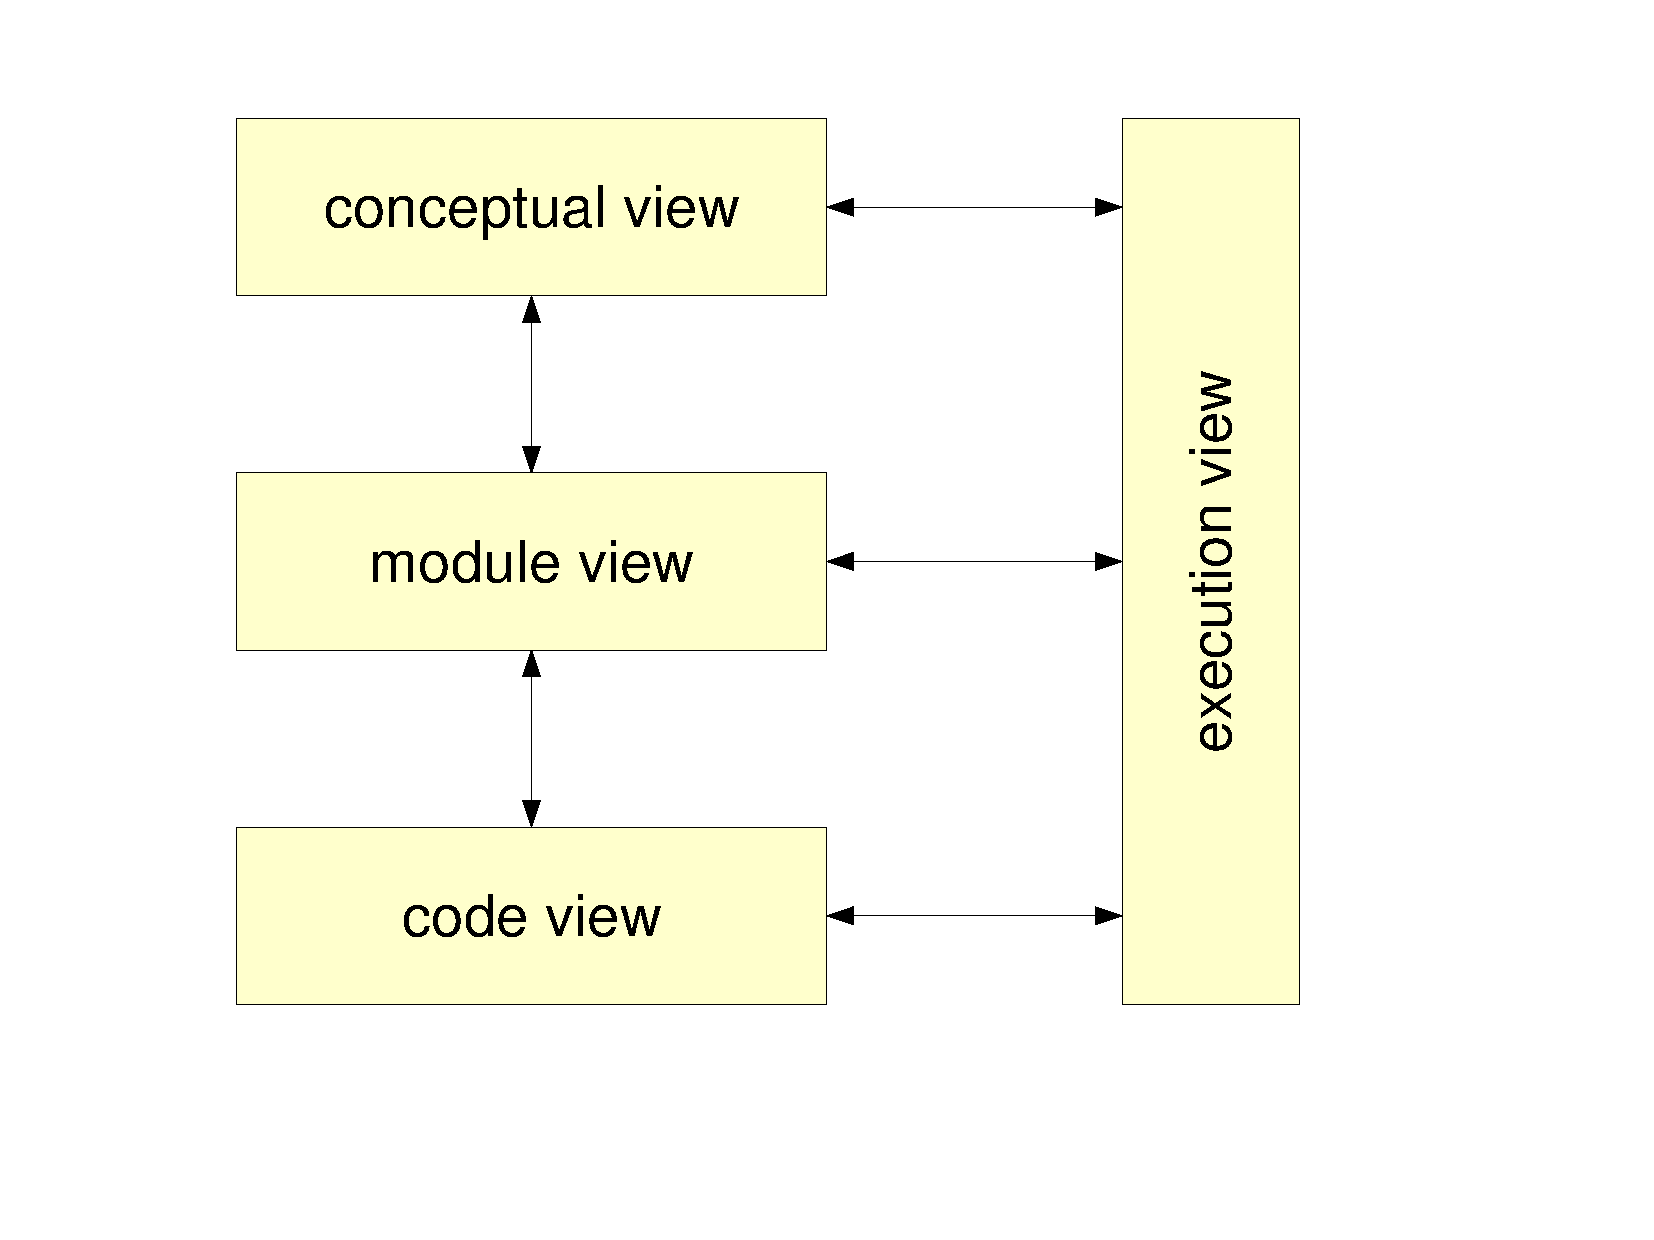
\includegraphics[scale=0.3,angle=-90]{graphic/fourviews.pdf}
        \caption{Four Views Model \cite{hofmeister}}
        \label{fourviews_figure}
    \end{center}
\end{figure}

The \emph{Four Views} model (figure \ref{fourviews_figure}) proposed by
\cite{hofmeister} is best suitable for representing architectures of systems that
are implemented in a procedural programming language. It contains four different
views that serve the following purposes:

\begin{itemize}
    \item[-] \emph{Conceptual View:} describe the major design elements of a
        system and the relations between them
    \item[-] \emph{Module View:} represent the decomposition of a system into
        modules that are grouped in layers
    \item[-] \emph{Code View:} organise source code into object code, libraries
        and binaries, and into corresponding version files and directories
    \item[-] \emph{Execution View:} map software to hardware and distribute
        software components
\end{itemize}

\begin{figure}[ht]
    \begin{center}
        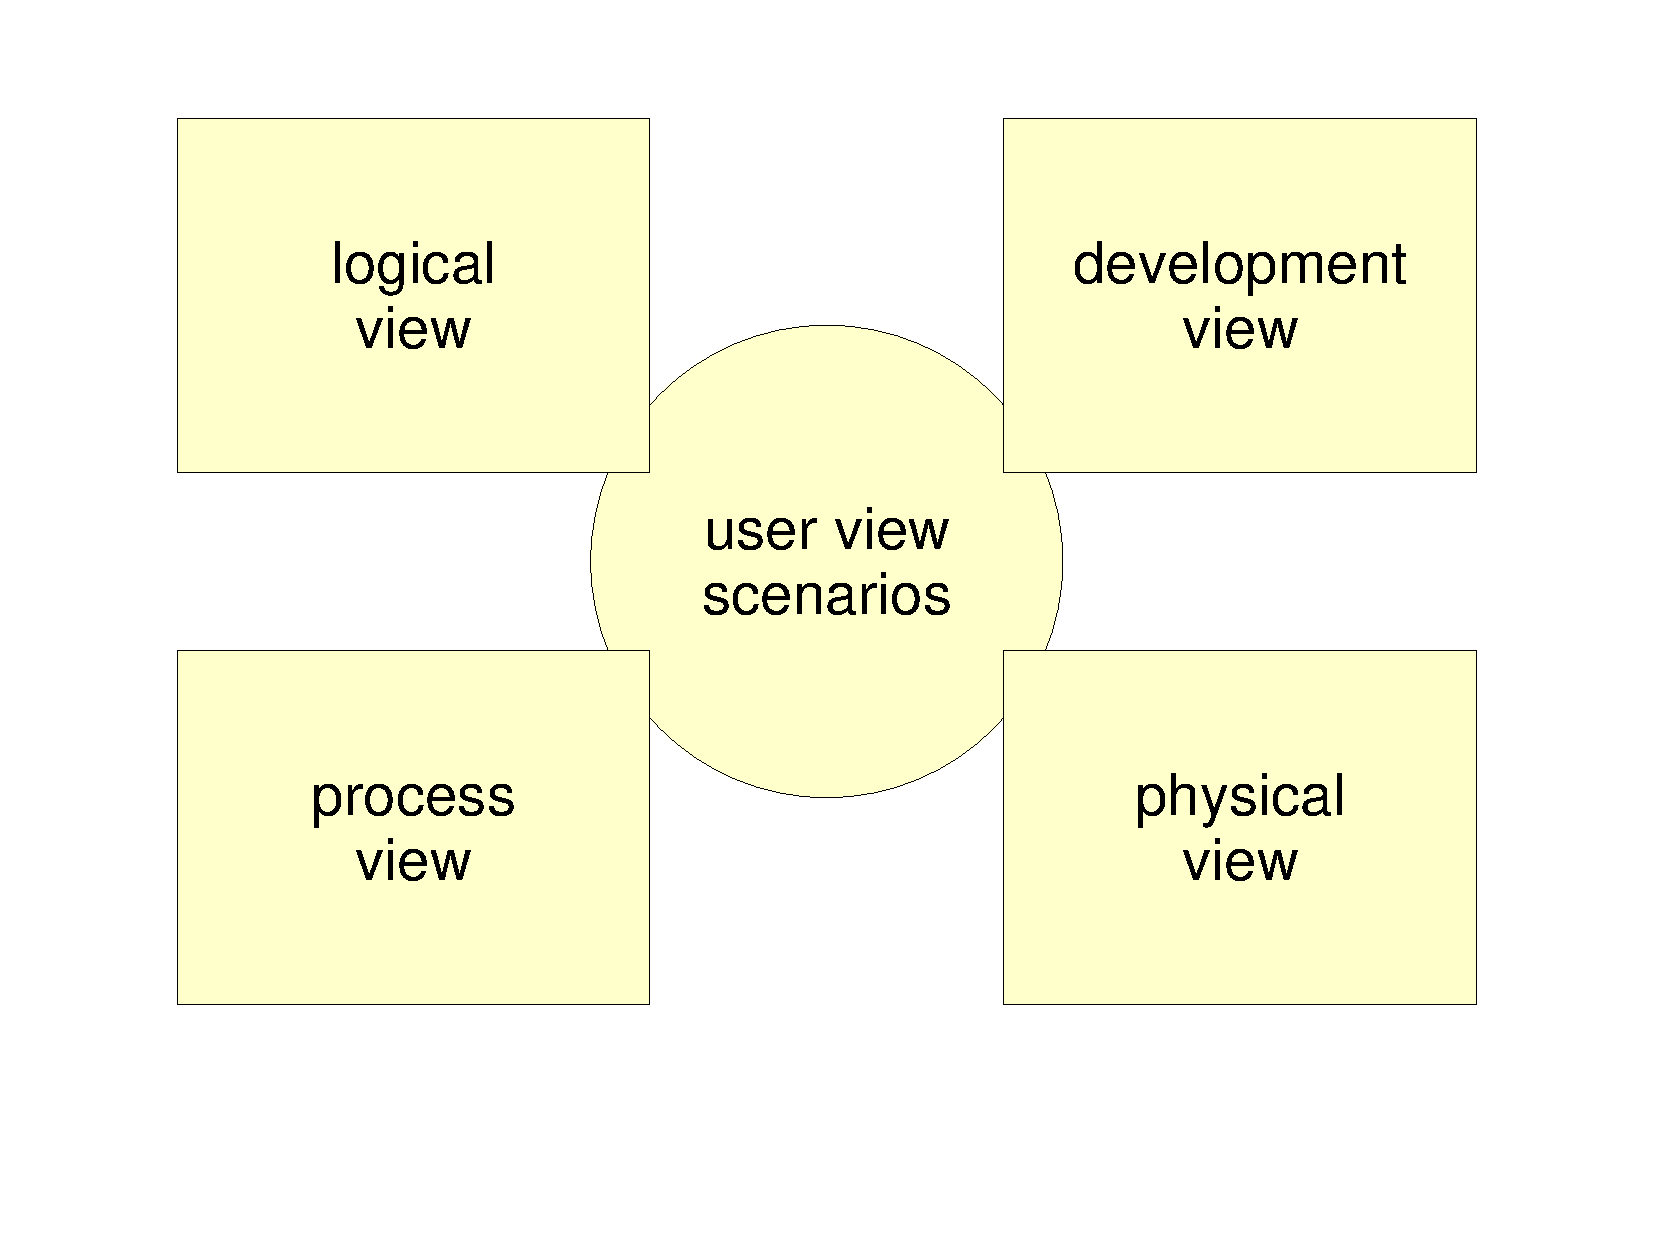
\includegraphics[scale=0.3,angle=-90]{graphic/4+1view.pdf}
        \caption{The 4+1 View Model of Architecture \cite{kruchten}}
        \label{4+1view_figure}
    \end{center}
\end{figure}

Architectures of systems that are implemented in an object-oriented way are better
represented by the \emph{4+1 View} model (figure \ref{4+1view_figure}), proposed by
\cite{kruchten} and embraced as part of the \emph{Rational Unified Process} (RUP)
\cite{rup}. It separates static and dynamic aspects and consists of five different
views, with the following purposes:

\begin{itemize}
    \item[-] \emph{Logical (Design) View:} map required system functionality to
        architecture elements
    \item[-] \emph{Development (Implementation) View:} focus on the actual
        software module organisation
    \item[-] \emph{Physical (Deployment) View:} assign software elements to
        concrete hardware nodes
    \item[-] \emph{Process View:} describe dynamic runtime behavior of the
        executed system
    \item[-] \emph{Scenarios (Use Case +1 View):} collect domain knowledge, from
        a user's view, and use them to validate and unify the other four views
\end{itemize}

Many other architecture modelling approaches like for instance the
\emph{Architecture Description Languages} (ADL), some representatives of which
are described in \cite{garlan, clements}, exist but are outside the scope of
this work and not elaborated further here, because the following two chapters
were created according to the \emph{4+1 View Model of Architecture}. Two
simplifications are made, however: The \emph{Physical-} also includes the
\emph{Process View} (chapter \ref{physical_architecture_heading}), because
processes are considered as communicating systems running on physical machines,
and the \emph{Logical-} also contains the \emph{Development View} (chapter
\ref{logical_architecture_heading}), because logical models represent
abstractions at different stages of software development. \emph{Scenarios} are
not considered since they belong to requirements engineering whose techniques
are not a topic of this work.

